\chapter{Budicí signál}

\section{Základní požadavky na vlastnosti budicího signálu}
Budicí signál musí splňovat jisté podmínky, aby jej bylo možné použít pro charakterizaci měřeného systému. Následuje formulace základních kritérií pro výběr vhodného budicího signálu.

\begin{itemize}
	\item
	\textbf{Fyzikální realizovatelnost}\\*
	Vzhledem k tomu, že navrhované zařízení musí být realizovatelné, je nezbytné, aby i budicí signál byl fyzikálně realizovatelný. Vzhledem k fyzikálním a praktickým omezením (existence materiálové disperze, nemožnost vytvoření nekonečně velkého proudu, neexistuje bezkapacitní prostředí, neexistuje bezindukční vedení, neexistuje zdroj schopný dodat nekonečné množství energie) není možné vytvořit nespojitý signál. Derivace napětí takovéhoto signálu tedy nemůže být nekonečná. Nespojité signály je tak možné pouze aproximovat spojitými signály, což omezuje například délku a strmost náběžných hran v těchto aproximovaných nespojitostech. Toto fyzikální omezení tedy omezuje frekvenční spektrum takového budicího signálu, zejména jeho šířku.
	
	\item
	\textbf{Spektrální požadavky}\\*	
	Spektrum budicího signálu by mělo být pokud možno konstantní a co nejširší. Neobsahuje-li budicí signál nějakou část spektra, není možné otestovat odezvu systému na tuto část spektra a plně tedy charakterizovat měřený systém. Důvod pro požadavek na rovné spektrum vyplývá z omezeného dynamického rozsahu reflektometru - pokud by část spektra měla příliš malou úroveň, bylo by měření v této části spektra buď více zatížené šumem, případně až neměřitelné. V případě měření některých systémů může být výhodné používat úzkopásmový signál, například při měření části systému nacházející se za pásmovou propustí. V takovém případě by mohla být odezva od části systému za pásmovou propustí maskována mnohem silnějším odrazem od propusti. Jedná se však o specifický případ, který je možné vyřešit i jinými metodami, například redukcí odrazu v nechtěném pásmu \cite{sincgausstdr}. Pro zcela obecné použití by měl být širokopásmový signál vhodnější.
	
	\item
	\textbf{Jednoduchost}\\*	
	Zvolený budicí signál by měl být jednoduchý na vytvoření. Se složitostí signálu může růst složitost zapojení, které by ho mělo generovat, jeho fyzická velikost, případně i náklady na takové zařízení.	

	\item
	\textbf{Rozlišitelnost budicího signálu od odrazů}\\*	
	Budicí signál musí být rozlišitelný od odrazů. Kupříkladu pro buzení periodickým signálem by mělo platit, že odezva měřeného systému na budicí signál musí být kratší než perioda budicího signálu. V opačném případě by se překrývala část odezvy s odezvou od další periody budicího signálu.
\end{itemize}

\section{Výběr budicího signálu a možnosti jeho syntézy}
V této části jsou uvedeny možné podoby budicích signálů a obecné možnosti jejich syntézy. Zároveň jsou zde diskutovány jejich vlastnosti a možnosti následného zpracování. U signálů jsou uvedeny i již existující implementace reflektometrů s těmito budicími signály.

\begin{itemize}
	\item
	\textbf{Diracovo delta}\\*	
	\begin{figure}[htbp]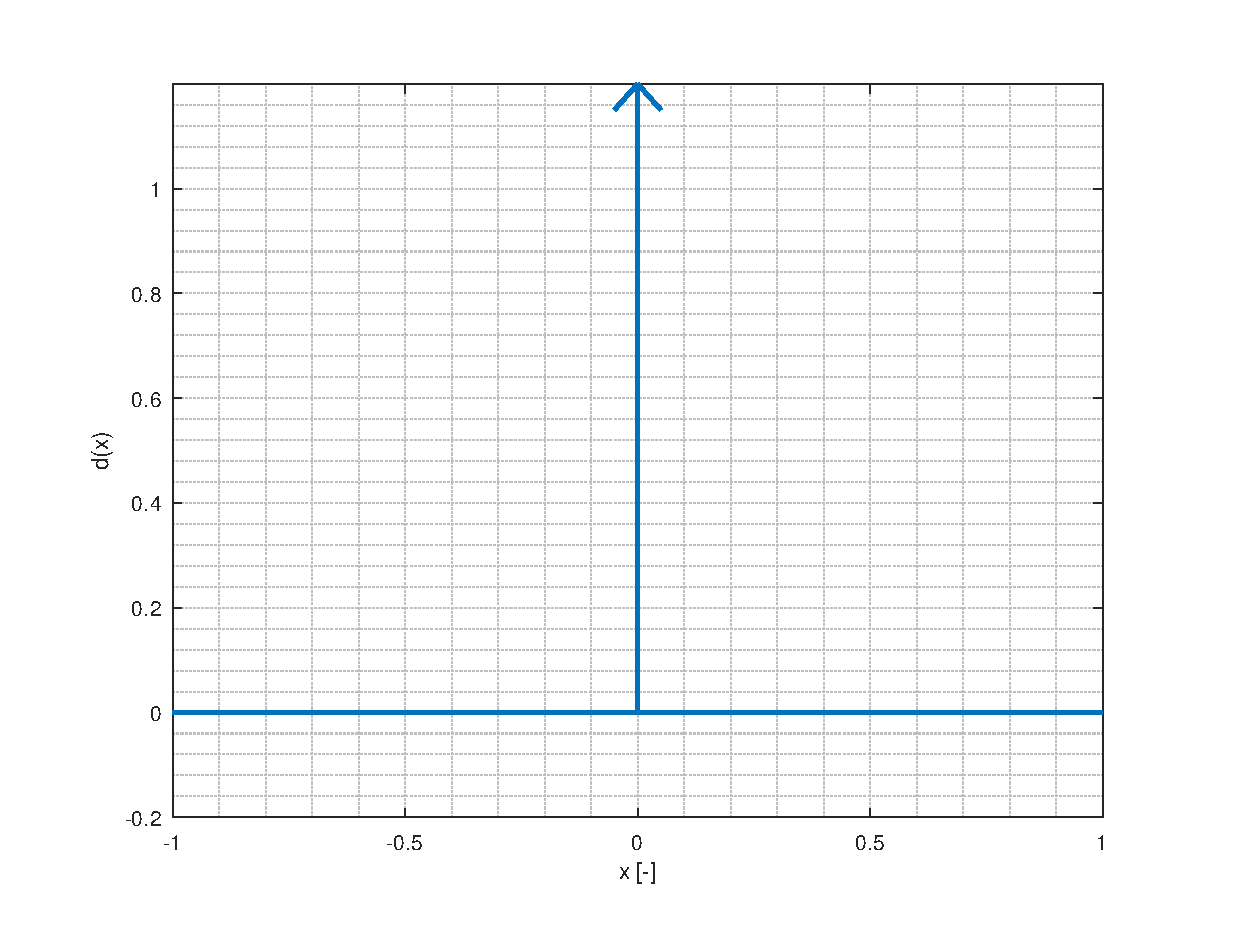
\includegraphics[width=\textwidth,keepaspectratio]{images/dirac.eps}\caption{Diracovo delta.}\label{dirac}\end{figure}		
	Diracovo delta (na obr. \ref{dirac}) je velice jednoduchý signál, který je jedním z ideálních budicích signálů, jeho spektrum je konstanta, má tedy neomezenou šířku frekvenčního pásma. Odezva na Diracovo delta odpovídá impulzní odezvě systému.  Bohužel není fyzikálně realizovatelný, jak je shrnuto v předchozí části textu, neboť je nespojitý a vyžaduje nekonečně rychlé změny napětí a proudu v obvodu. Je tedy možné pouze jej aproximovat, čímž se změní jeho spektrum. Výsledný signál bude mít spektrum odpovídající spektru Diracova delta filtrovaného dolní propustí, čímž se jeho šířka pásma omezí na konečnou velikost. Možná podoba takového signálu je Gaussův pulz na obr. \ref{gauss}.
	
	\begin{figure}[htbp]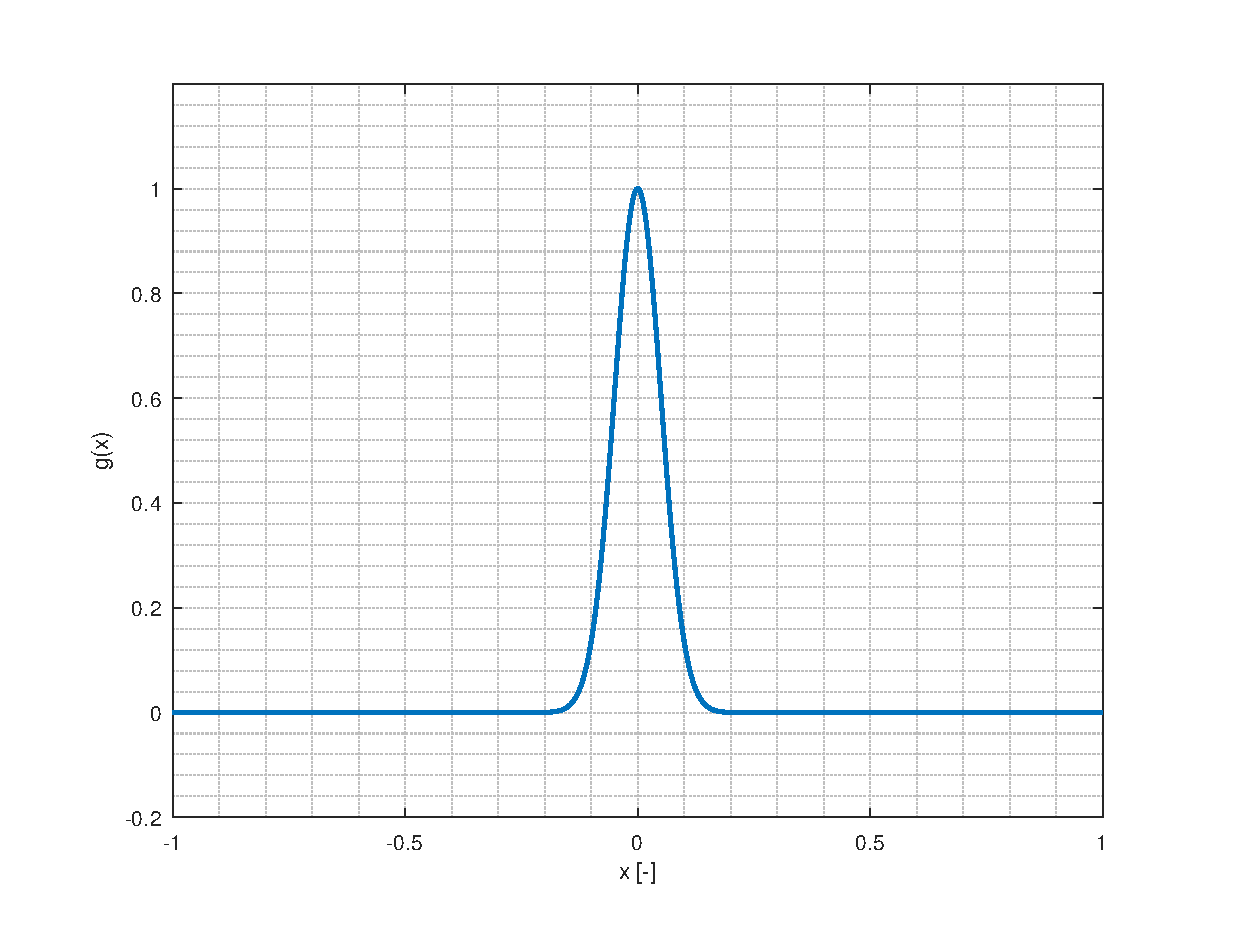
\includegraphics[width=\textwidth,keepaspectratio]{images/gauss.eps}\caption{Gaussův pulz, variance=0.05.}\label{gauss}\end{figure}			
	
	Aproximaci Diracova delta je možné vytvořit pomocí lavinových generátorů impulzů \cite{AN72LT}, \cite{AN94LT}. Pro dosažení impulzu o délce menší než stovky pikosekund je možné použít kombinaci lavinového generátoru impulzů, \acrfull{SRD} a takzvané \gls{clipline} podle obr. \ref{clipline_generator} \cite{S-4manual} \cite{S-1manual}. Takové řešení je však již prostorově náročné, protože vyžaduje zdroj lavinového napětí, transformátory a zkratovací vedení.
	
	\begin{figure}[htbp]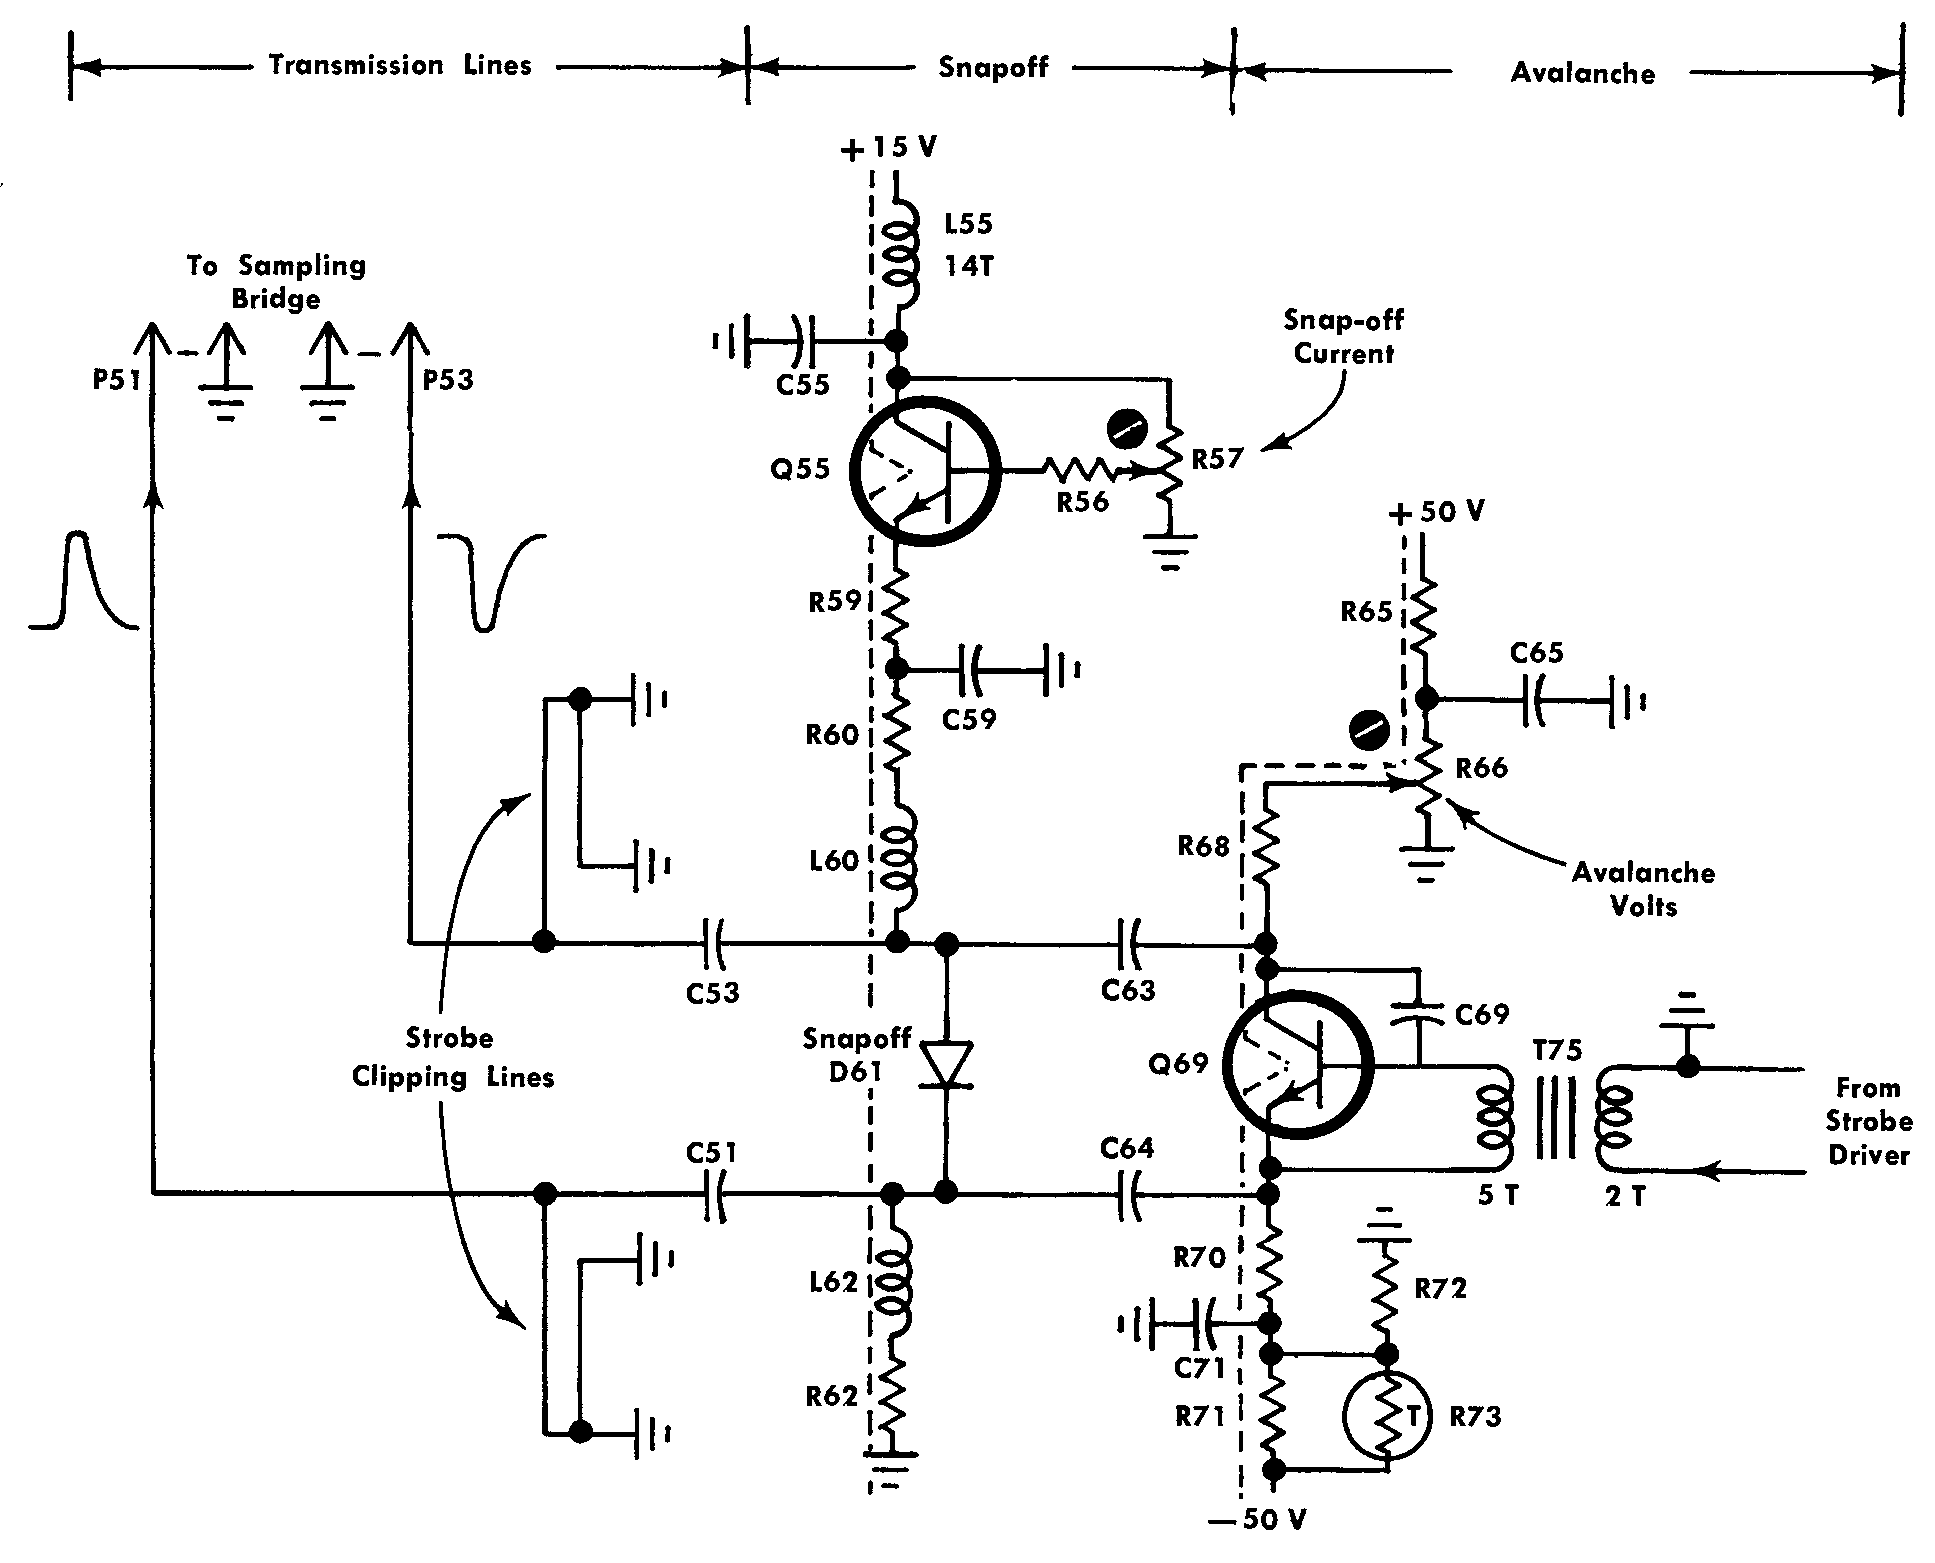
\includegraphics[width=\textwidth,keepaspectratio]{images/clipline_generator.png}\caption{Jehlový generátor s lavinovým generátorem, \acrshort{SRD} a zkratovacím vedením \cite{S-1manual}.}\label{clipline_generator}\end{figure}			
	
	\item
	\textbf{Jednotkový skok}\\*
	\begin{figure}[htbp]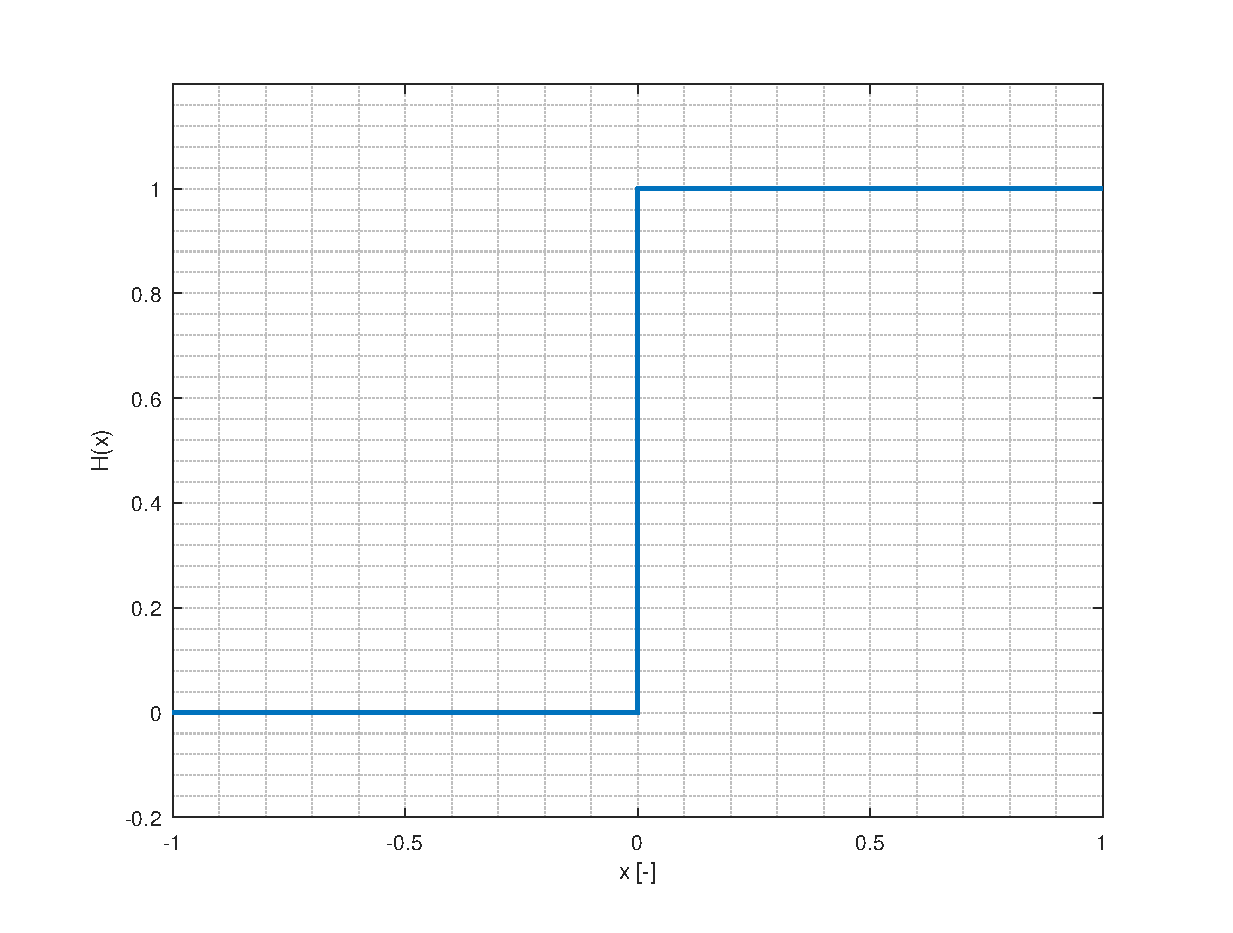
\includegraphics[width=\textwidth,keepaspectratio]{images/unitstep.eps}\caption{Jednotkový skok.}\label{unitstep}\end{figure}		
	Jednotkový skok na obr. \ref{unitstep} odpovídá časovému integrálu Diracova delta
	\begin{equation}
		H(x)=\int_{-\infty}^x \delta(t) dt.
	\end{equation} Opět se jedná o nespojitý signál, který nejde realizovat, jen aproximovat. Reálná aproximace jednotkového skoku je například chybová funkce $\erf(x)$ na obr. \ref{errorfunction}.
	
	\begin{figure}[htbp]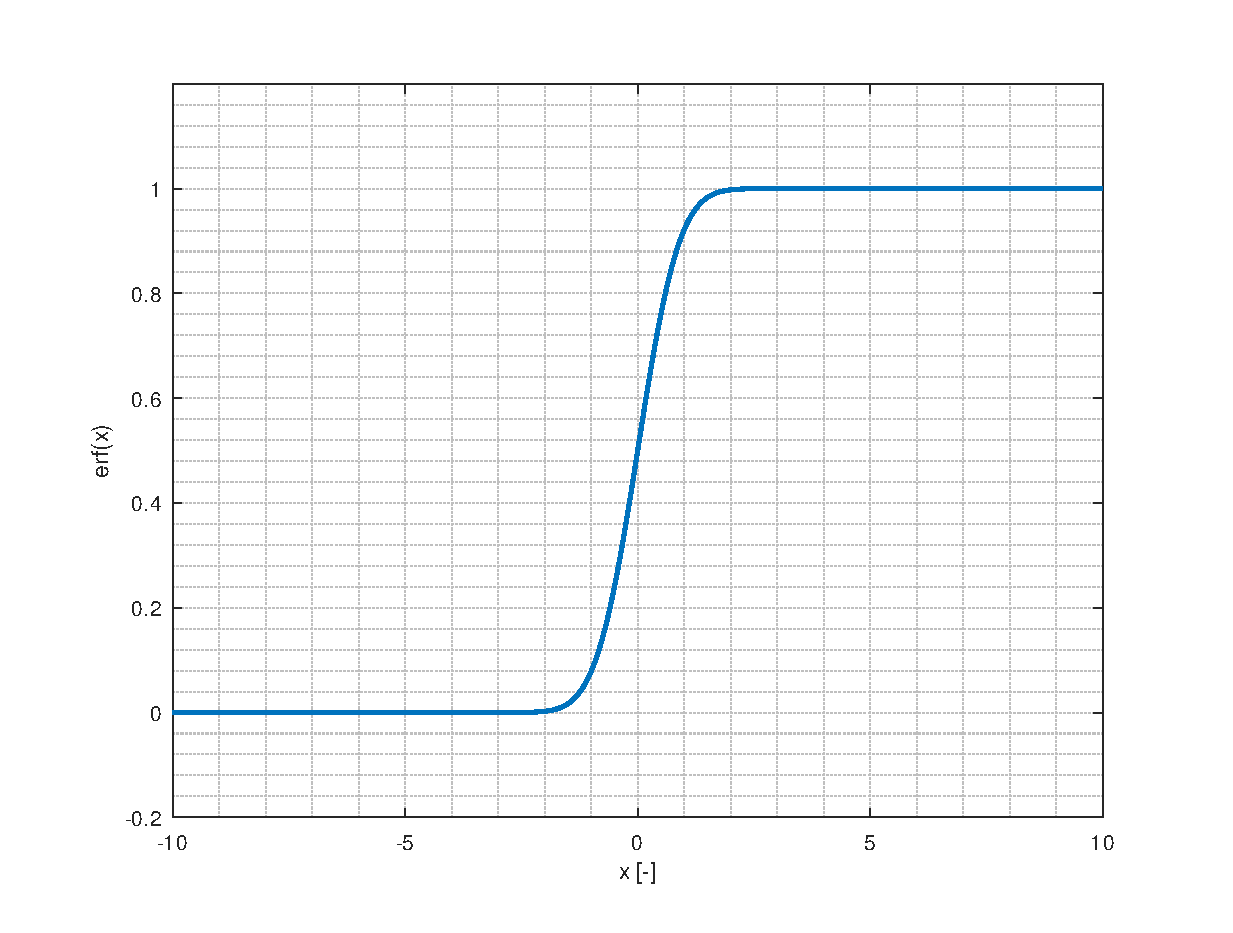
\includegraphics[width=\textwidth,keepaspectratio]{images/erf.eps}\caption{Chybová funkce.}\label{errorfunction}\end{figure}		
		
	Tento budicí signál je možné jednoduše generovat pomocí rychlých logických obvodů. Moderní logické obvody používané pro vysokorychlostní spoje (\acrshort{SATA}, \acrshort{SAS}, \acrshort{USB}\,3, \acrshort{PCI-E}) v řádu jednotek \si{\giga\bit\per\second} již mají náběžné hrany o délce kratší než 100 ps \cite{SY54017datasheet}, \cite{SN75LVCP600Sdatasheet}, \cite{SN65LVPE501datasheet}, \cite{TUSB1002Adatasheet}. Vzhledem k tomu, že pro převod skokové odezvy na impulsní je možné použít jednoduchý vztah
	\begin{equation}
	h(t)=\dv{a(t)}{t},
	\end{equation} a že je syntéza jednotkového skoku možná přímo pomocí logického obvodu, je výhodnější použít jednotkový skok než Diracovo delta. Pravděpodobně z těchto důvodů se u běžných reflektometrů používá právě jednotkový skok jako budicí signál.
	
	\item
	\textbf{Funkce $\boldsymbol{\sinc(x)}$}\\*	
	\begin{figure}[htbp]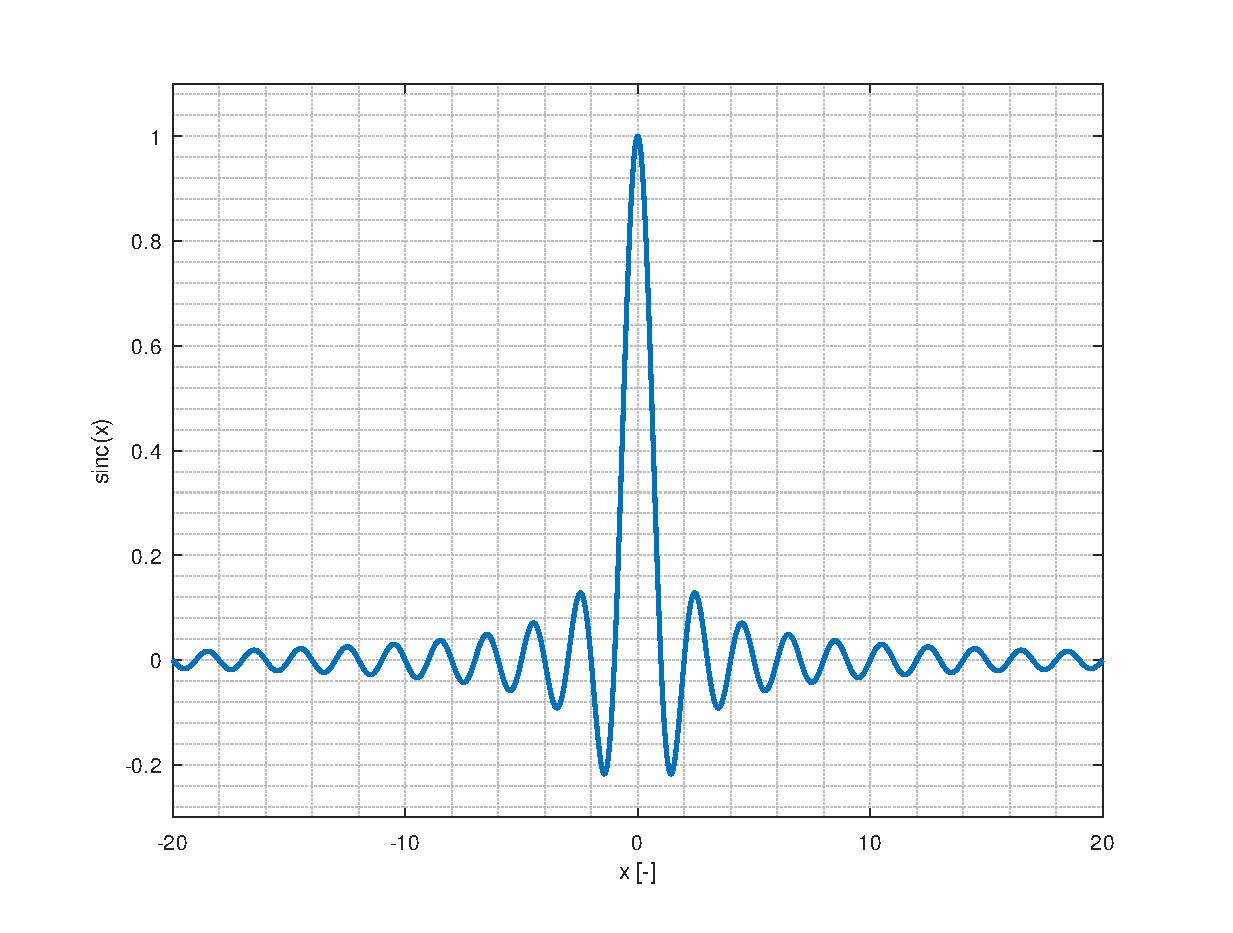
\includegraphics[width=\textwidth,keepaspectratio]{images/sinc.eps}\caption{Funkce $\sinc(x)$.}\label{sinc}\end{figure}		
	
	Další možný budicí signál je funkce $\sinc(x)$ na obr. \ref{sinc}. Tato je již idealizovaně fyzikálně proveditelná (musela by být nekonečně dlouhá), spektrum funkce je konstantní až do mezní frekvence, dále je nulové. Vzhledem k ostrému omezení spektra bohužel není možné změřenou odezvu převést na impulsní odezvu, což komplikuje další zpracování. Autokorelace této funkce je opět $\sinc(x)$, není tedy možné takto jednoduše takovouto odezvu analyzovat.
	
	Pro vytvoření průběhu funkce $\sinc(x)$ je možné modulovat harmonický signál obálkou \cite{sincgausstdr}, ovšem taková obálka by musela být přesně synchronizována s nosným harmonickým signálem, aby nedocházelo ke zkreslení spektra. Jedna z možností, jak přesně simulovat tuto funkci je přímá digitální syntéza, pro tu by ovšem bylo nezbytné použít obvod \acrshort{DDS} s hodinovou frekvencí nejméně dvakrát větší než požadované pásmo, tedy vyšší jednotky GHz. Tento signál nenabízí tedy ani snadnou implementaci, ani vhodné vlastnosti pro použití jako buzení.
	
	\item
	\textbf{Bílý šum}\\*	
	\begin{figure}[htbp]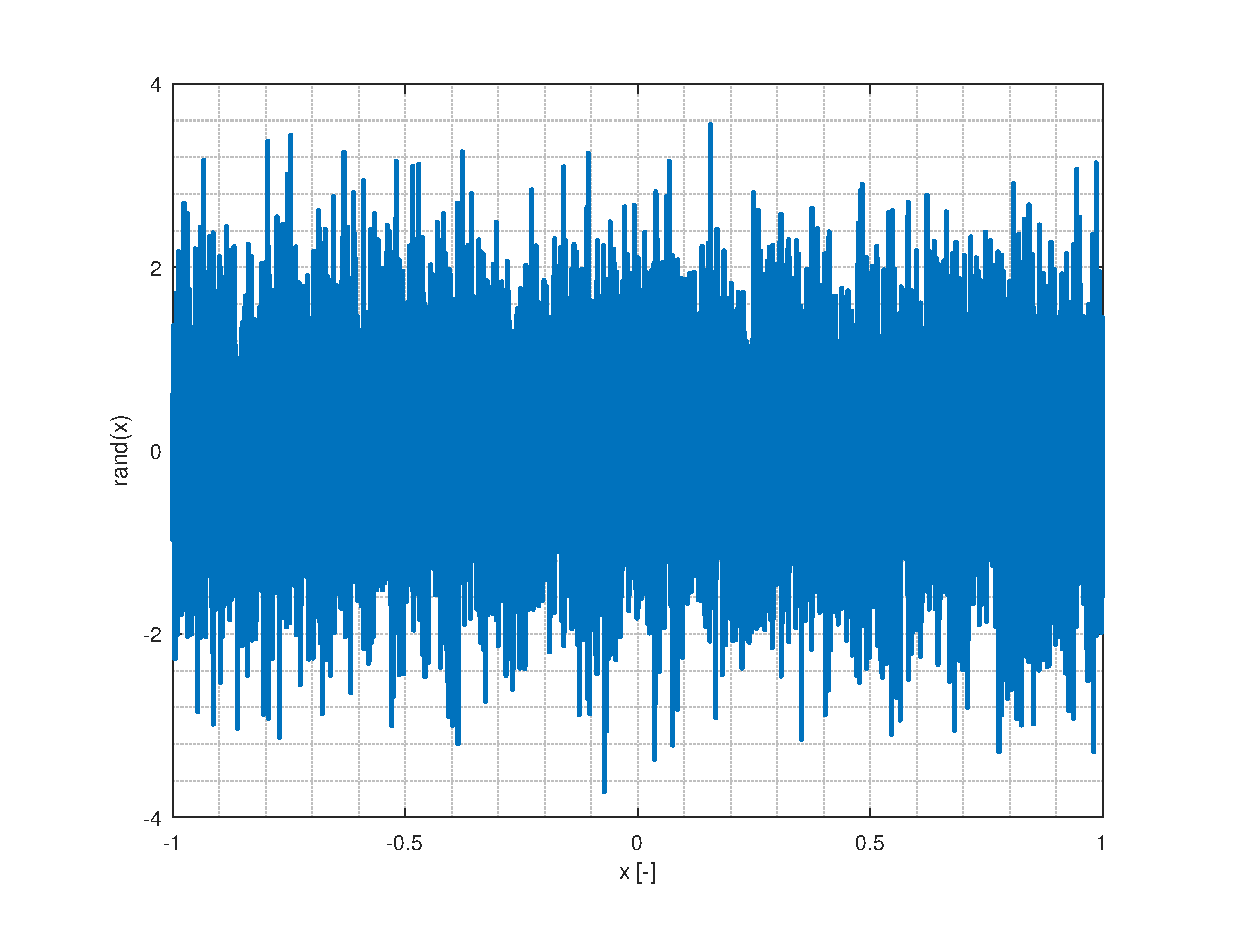
\includegraphics[width=\textwidth,keepaspectratio]{images/whitenoise.eps}\caption{Diskrétní bílý šum.}\label{whitenoise}\end{figure}			
	Při použití bílého šumu (obr. \ref{whitenoise}) je možné získat impulsní odezvu pomocí autokorelace odezvy soustavy. Taková operace zároveň může potlačit nežádaný šum. Pro použití bílého šumu by ale bylo nezbytné, aby budicí šum byl rozlišitelný od šumu nežádaného. Toho lze dosáhnout například zapínáním a vypínáním budicího šumu.
	
	\begin{figure}[htbp]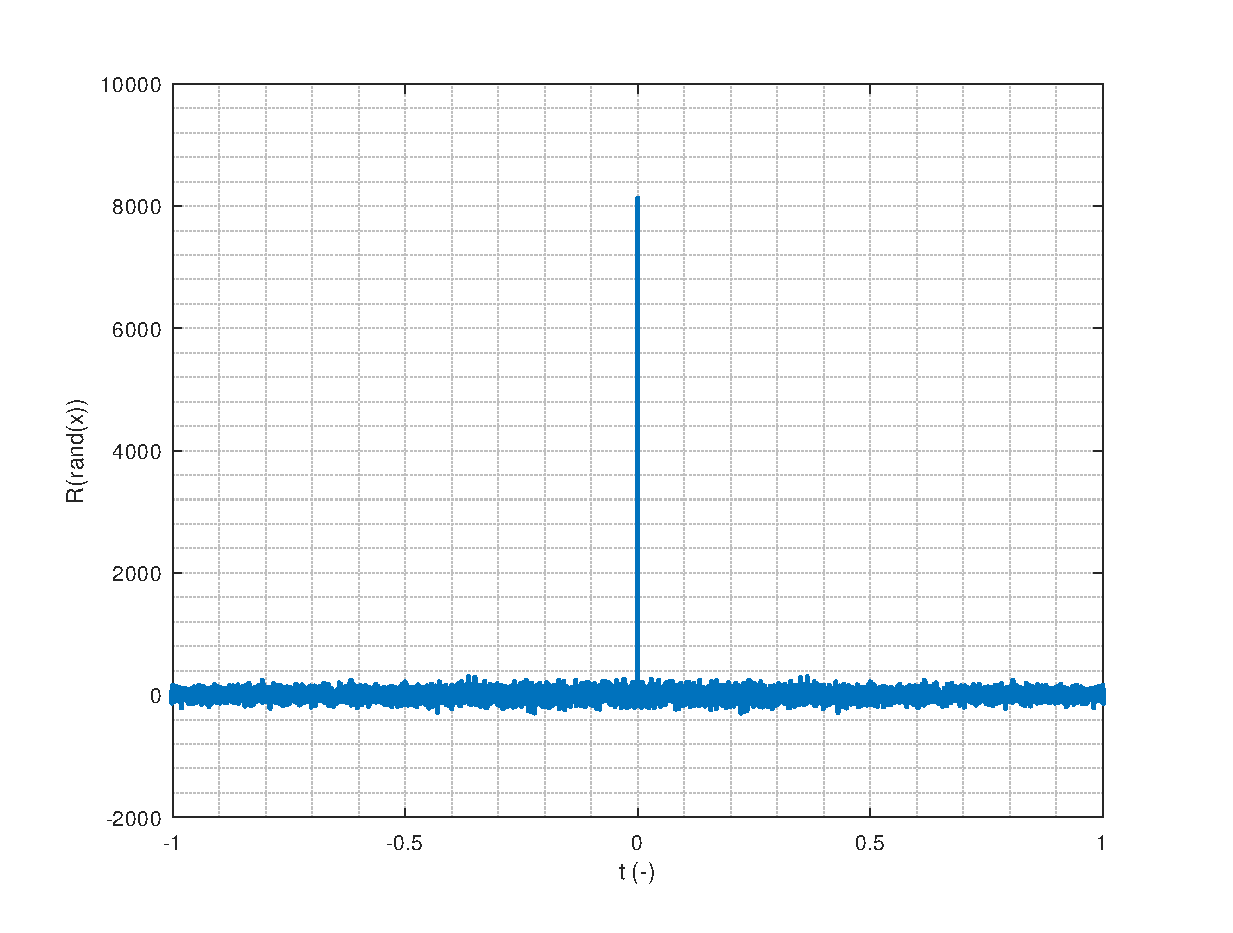
\includegraphics[width=\textwidth,keepaspectratio]{images/whitenoisecorr.eps}\caption{Autokorelace diskrétního bílého šumu z \ref{whitenoise}.}\label{whitenoisecorr}\end{figure}		
	
	Širokopásmový šum je také možné jednoduše vytvořit, například pomocí šumových diod. Modulaci tohoto šumu je možné provádět například pomocí polovodičových mikrovlnných přepínačů. Takový budicí signál je tedy možné jednoduše vytvořit i zpracovávat. Podstatná nevýhoda bílého šumu spočívá v náhodnosti, a z toho vyplývající neperiodicity, kvůli které není možné odezvu systému na takový signál měřit v ekvivalentním čase, jen v reálném čase. Je možné ovšem rovnou měřit autokorelaci, tedy násobením odezvy systému se zpožděnou kopií, kterou je možné vzorkovat pomalu. Autokorelace diskrétního bílého šumu se nachází na obr. \ref{whitenoisecorr}. Bohužel takový přístup vyžaduje použití zpožďovacího vedení s proměnnou délkou, které musí být buď vytvořeno jako mechanický pohyblivý díl nebo jako vedení s velkým množstvím odboček, pak ale je časový krok měření omezen polohou odboček a celková délka měření je omezena délkou vedení \cite{noisedomainreflectometry}. Tuto metodu měření je možné použít pro měření na vedení, na kterém se nachází aktivní zařízení, protože nežádané signály je možné do velké míry odfiltrovat autokorelací. Tato metoda může být tedy výhodná pro měření na předem známých systémech (pevná nehybná vedení), například ve strojích, továrnách, dopravních prostředcích, pro obecné použití se však nezdá být praktická. 
	
	\item
	\textbf{Deterministický šum}\\*
	Za deterministický šum je možné považovat například vedení, které slouží k digitální komunikaci, přičemž obsah posílaných zpráv je známý nebo se tyto zprávy opakují. Pro měření touto metodou je však nezbytná znalost konkrétního měřeného systému \cite{noisedomainreflectometry}, nejde tedy o všeobecně použitelou metodu. 
\end{itemize}

\section{Zvolený budicí signál a obvodové řešení}
Pro jednoduchost syntézy a dobré vlastnosti byl vybrán jednotkový skok. Kvůli rychlostním požadavkům není možné použít klasické logické obvody z řad \acrshort{TTL}, \acrshort{CMOS}, \acrshort{LVCMOS}, \acrshort{HCMOS}, \acrshort{ECL} apod. kvůli velké délce náběžné hrany \cite{subnanosecondgeneratorcomparison}. U těchto technologií je náběžná hrana zpravidla delší než \SI{1}{\nano\second}. Vzhledem k vývoji dnešní techniky, zejména v oblasti vysokorychlostních digitálních přenosů, však již existují velice rychlé logické obvody schopné dosahovat náběžných hran o délce kratší než \SI{100}{\pico\second}. Ve všech dnešních počítačích se již nacházejí technologie jako \acrshort{USB}\,3, \acrshort{HDMI} nebo Display Port, \acrshort{PCI-E}, \acrshort{SATA} nebo \acrshort{SAS} (v serverech), které právě takové obvody vyžadují, díky čemuž jsou dnes již tyto obvody velmi levné. Tyto technologie jsou zpravidla pevně spojeny s metodou signalizace. Používané metody jsou vždy symetrické kvůli šumové odolnosti, používají signalizaci o rozkmitu řádově stovek milivoltů kvůli rychlosti a vyzařování do okolí. 

Běžně používané signalizační technologie:
\begin{itemize}
	\item
	\textbf{\acrshort{LVPECL}}\\*	
		Nízkonapěťová varianta dřívějšího \acrshort{ECL}, která je navíc referencovaná vůči kladnému napájecímu pólu. Vnitřní zapojení je uvedeno na schématu \ref{lvpecl_output}. Jsou navrženy pro připojení k impedanci \SI{50}{\ohm}, bohužel výstupní budiče jsou zapojeny jako emitorové sledovače \cite{lvpecl_vml_cml_lvds_interfacing}, jsou tedy silně nelineární, nemají definovanou impedanci a nejsou tedy vhodné jako budicí obvod do reflektometru, neboť v reflektometru se vyžaduje dobré přizpůsobení měřicího portu, tedy jeho impedance musí být přesně definovaná a konstantní, navíc není žádoucí, aby se měřicí port choval nelineárně.
	
		\begin{figure}[htbp]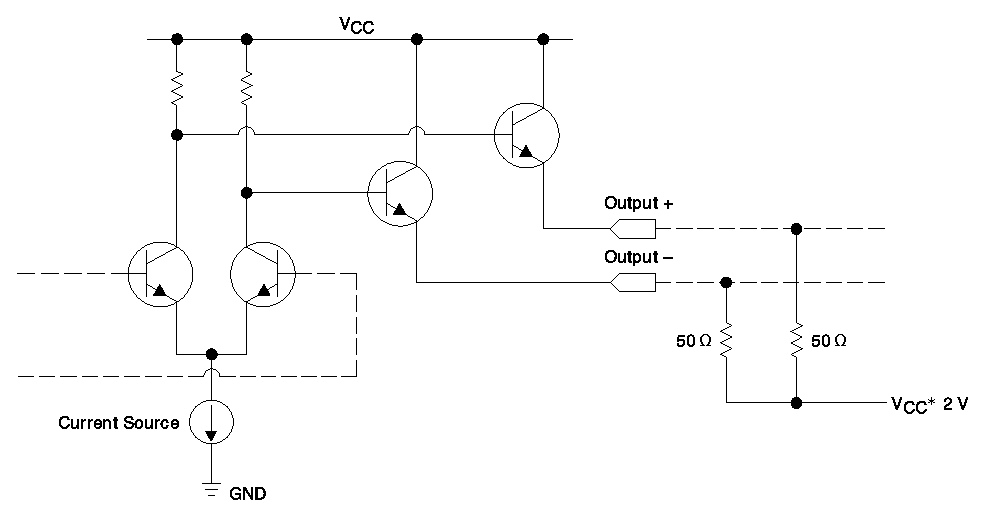
\includegraphics[width=\textwidth,,height=10cm,keepaspectratio]{images/lvpecl_output.eps}\caption{Typické zapojení LVPECL výstupu, převzato \cite{lvpecl_vml_cml_lvds_interfacing}.}\label{lvpecl_output}\end{figure}		
		
	\item
	\textbf{\acrshort{LVDS}}\\*
		Tato signalizace se běžně používá pro přenos obrazu po \acrshort{HDMI} nebo Display Port. Se zmenšeným rozkmitem (\SI{250}{\milli\volt}) se používá i pro \acrshort{SATA} a \acrshort{SAS}.  Vnitřní zapojení je uvedeno na schématu \ref{lvds_output}. Výstupní budiče jsou zapojeny jako \acrshort{CMOS} push-pull budiče \cite{lvpecl_vml_cml_lvds_interfacing} zapojené do drainů tranzistorů, velice podobné jsou i budiče technologie \acrshort{VML} \cite{lvpecl_vml_cml_lvds_interfacing} a \acrshort{HCSL}, očekává se diferenciální zakončení přibližně \SI{100}{\ohm}, případně $2\times\SI{50}{\ohm}$ s pevným středem. Tyto budiče by měly být méně nelineární než \acrshort{LVPECL}, opět však zpravidla není výstupní impedance garantována.
		
		\begin{figure}[htbp]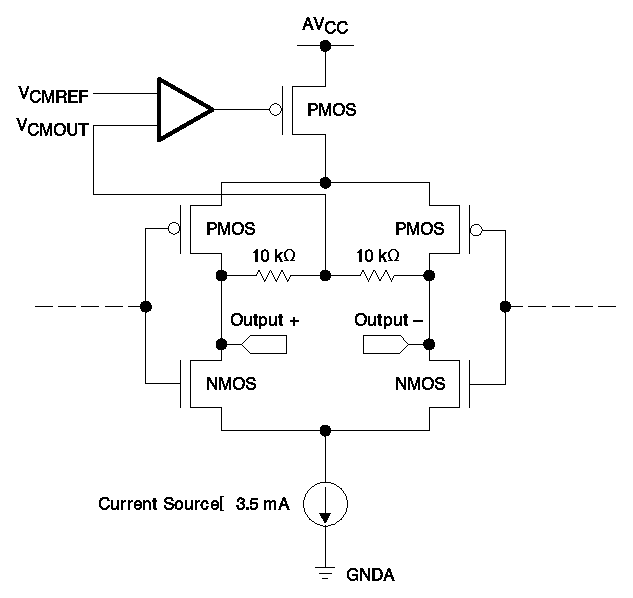
\includegraphics[width=\textwidth,height=8cm,keepaspectratio]{images/lvds_output.eps}\caption{Typické zapojení \acrshort{LVDS} výstupu, převzato z  \cite{lvpecl_vml_cml_lvds_interfacing}.}\label{lvds_output}\end{figure}	

	\item
	\textbf{\acrshort{CML}}\\*
		\acrshort{CML} je signalizační standard používaný zejména pro přenos hodinových signálů. Vnitřní zapojení je uvedeno na schématu \ref{cml_output}. Výstupní budiče jsou zapojeny do kolektoru resp. drainu tranzistoru \cite{lvpecl_vml_cml_lvds_interfacing}, jsou terminovány na \SI{50}{\ohm}, tato hodnota a její tolerance bývá garantována \cite{SY54017datasheet}. Vzhledem k zapojení do kolektoru a interní terminaci je takovýto budič velice dobře přizpůsobený k \SI{50}{\ohm} vedení. 
	
		\begin{figure}[htbp]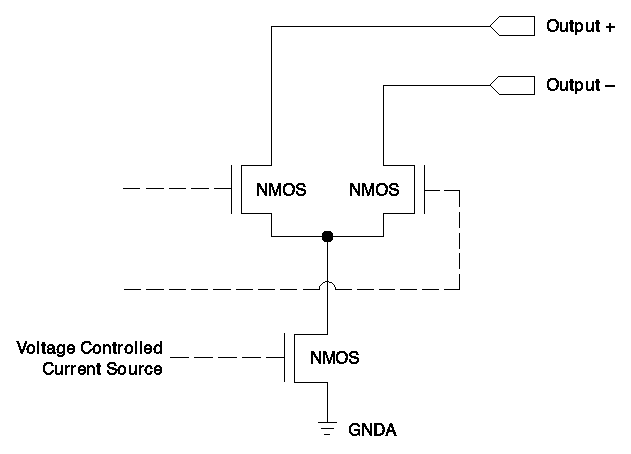
\includegraphics[width=\textwidth,height=8cm,keepaspectratio]{images/cml_output.eps}\caption{Typické zapojení \acrshort{CML} výstupu, převzato z \cite{lvpecl_vml_cml_lvds_interfacing}.}\label{cml_output}\end{figure}		
		
	\item
	\textbf{\acrshort{USB}}\\*
		Další signalizační standard používá například USB, ovšem standard \acrshort{USB}\,3.0 \cite{usb30standard} nespecifikuje přímo technologii, jak této signalizace dosáhnout. Vzhledem k této nejasnosti byly USB redrivery vyřazeny z výběru.
\end{itemize}

Kvůli dobrému přizpůsobení, linearitě a vysoké rychlosti byla zvolena technologie \acrshort{CML}. Další výhodou je, že některým \acrshort{CML} logickým členům je možné měnit napájecí napětí výstupních budičů \cite{SY54020datasheet}. Nejrychlejší dostupné \acrshort{CML} budiče mají typickou délku náběžné hrany \SI{60}{\pico\second} (garantovaný rozsah \mbox{\SIrange{30}{95}{\ps}}, uvádí se pro \mbox{\SIrange{20}{80}{\%}} konečného napětí) \cite{SY54020datasheet}, \cite{SY54017datasheet}. Jsou přímo určeny pro digitální přenosy o rychlostech v řádu \si{\gigabitpersecond}. Tyto budiče tedy splňují požadavek na šířku pásma budicího signálu.
Další důvod pro použití technologie \acrshort{CML} je ten, že \acrshort{SATA}/\acrshort{SAS}/\acrshort{USB} redrivery obvykle obsahují i logiku, která detekuje, zda je přítomen validní signál odpovídající danému přenosovému médiu a v případě, že jej nedetekují, přejdou do úsporného režimu. Přesná metoda, jak je toto spojení detekováno, není zpravidla popsána, hrozilo by tedy, že by se mohl redriver chovat nedefinovaně. Další problém těchto redriverů je to, že jsou určeny pro kompenzaci vlivu frekvenční charakteristiky a ztrát na FR-4 substrátu, takže výsledný signál není prostý obdélníkový průběh, ale složitější stupňovitý průběh jako na obr. \ref{redriver} \cite{SN75LVCP601datasheet}.

		\begin{figure}[H]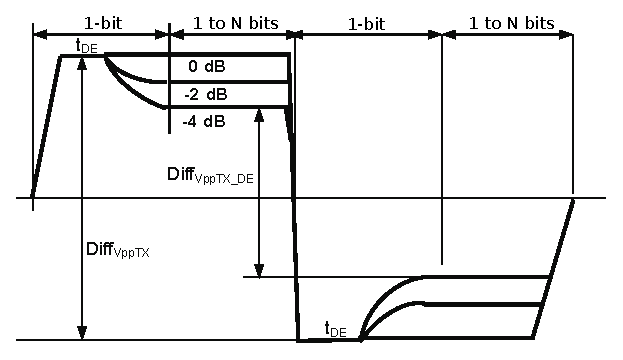
\includegraphics[width=\textwidth,height=6cm,keepaspectratio]{images/redriver.eps}\caption{Výstupní průběh \acrshort{SATA} redriveru \cite{SN75LVCP601datasheet}.}\label{redriver}\end{figure}		
